\chapter{Methodology}
\label{sec:methodology}

\section{System Design and Architecture}
This section outlines the full system architecture and implementation strategy behind the autonomous LEGO train prototype. The aim was to build a decentralized, modular, and voice-interactive control system driven by a local agentic LLM. Built entirely on a Raspberry Pi 4 without cloud dependencies, the system integrates the open source LangGraph framework, uses ZeroMQ, and lightweight ASR and vision tools to ensure autonomous behavior and safety. \\

The implementation process consists of the following steps:

\begin{enumerate}
    \item \textbf{Setting up the Raspberry Pi}: Establish a Raspberry Pi environment equipped with necessary libraries, including LangGraphs dependencies, ASR modules, ZMQ, and the open-source llama3-groq-tool-use with Ollama.
    \item \textbf{Developing the Agent}: Create functions within the LangGraph framework to interpret user input and translate them into corresponding commands for the LEGO train. This includes understanding natural language, state awareness, and decision-making logic.
    \item \textbf{Integrating Speech Recognition}: Implement ASR capabilities to recognize voice commands issued by the user. This involves setting up and train the model to ensure that it accurately interprets commands related to the operation of the train.
    \item  \textbf{Testing Control Logic}: Establish the control server logic for the LEGO train, which will handle commands from both the agent and the user interface. This server will continuously monitor the actions of the train and report its status to the agent in real time.
    \item  \textbf{Implementing Safety Measures:} To ensure safety during operation, the agent must react to disturbances in its environment, such as unexpected objects on the track. The system incorporates an object detection framework that triggers an emergency stop command when an obstacle is detected.
\end{enumerate}

\subsection{System Overview}

\begin{figure}[H]
\label{fig:system_architecture}
    \centering
    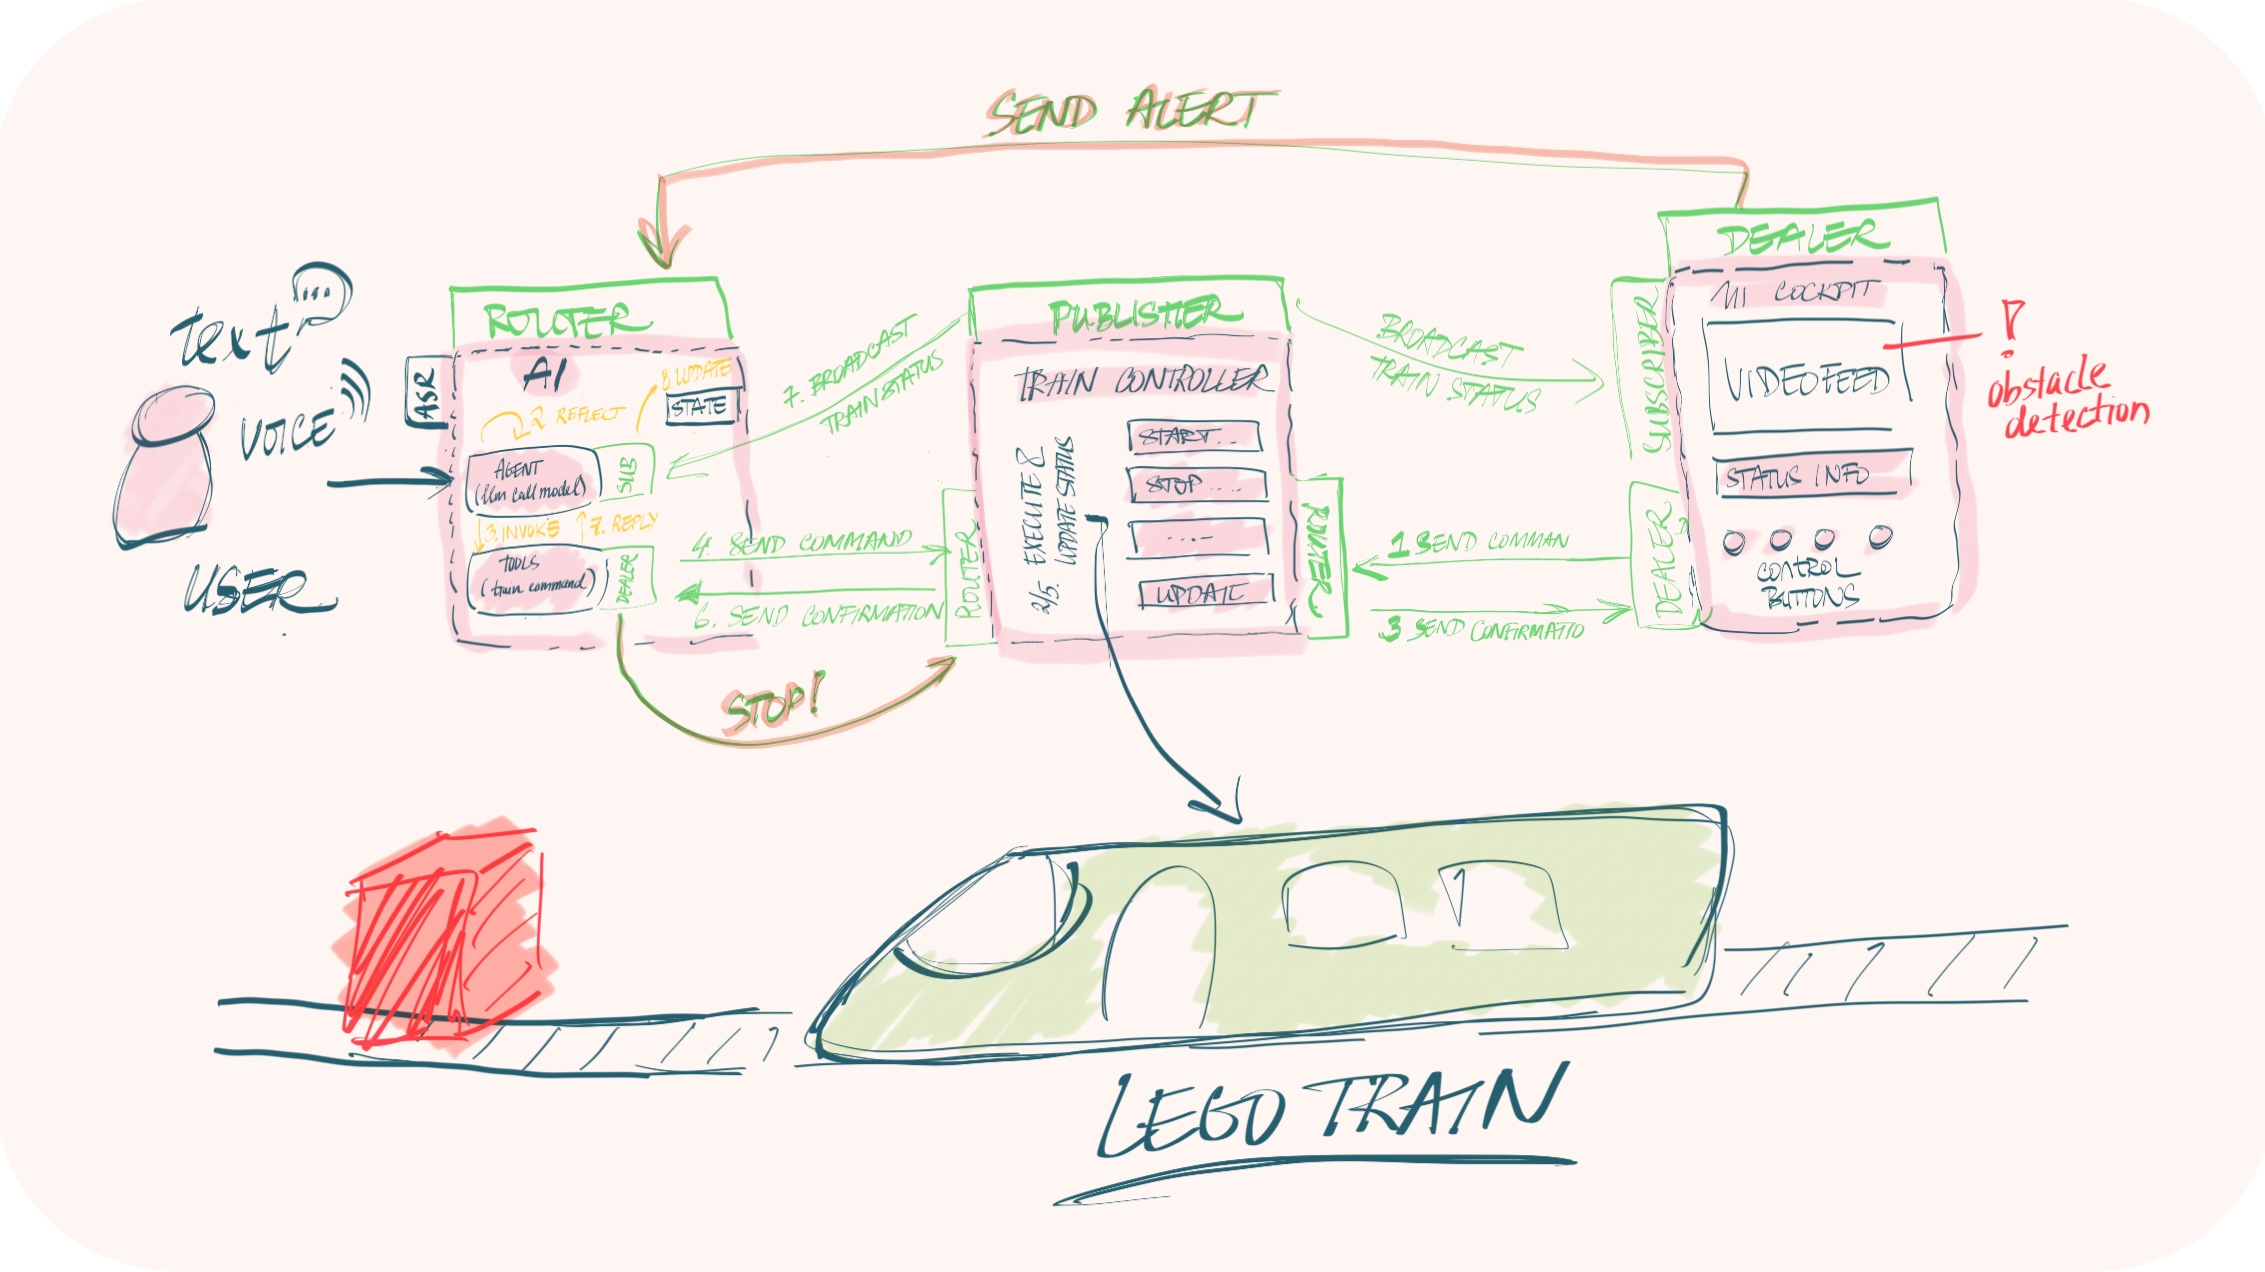
\includegraphics[width=\textwidth]{docs/system.jpg}
    \caption{System Architecture}
\end{figure}

\begin{figure}[H]
    \centering
    \label{fig:graph}
    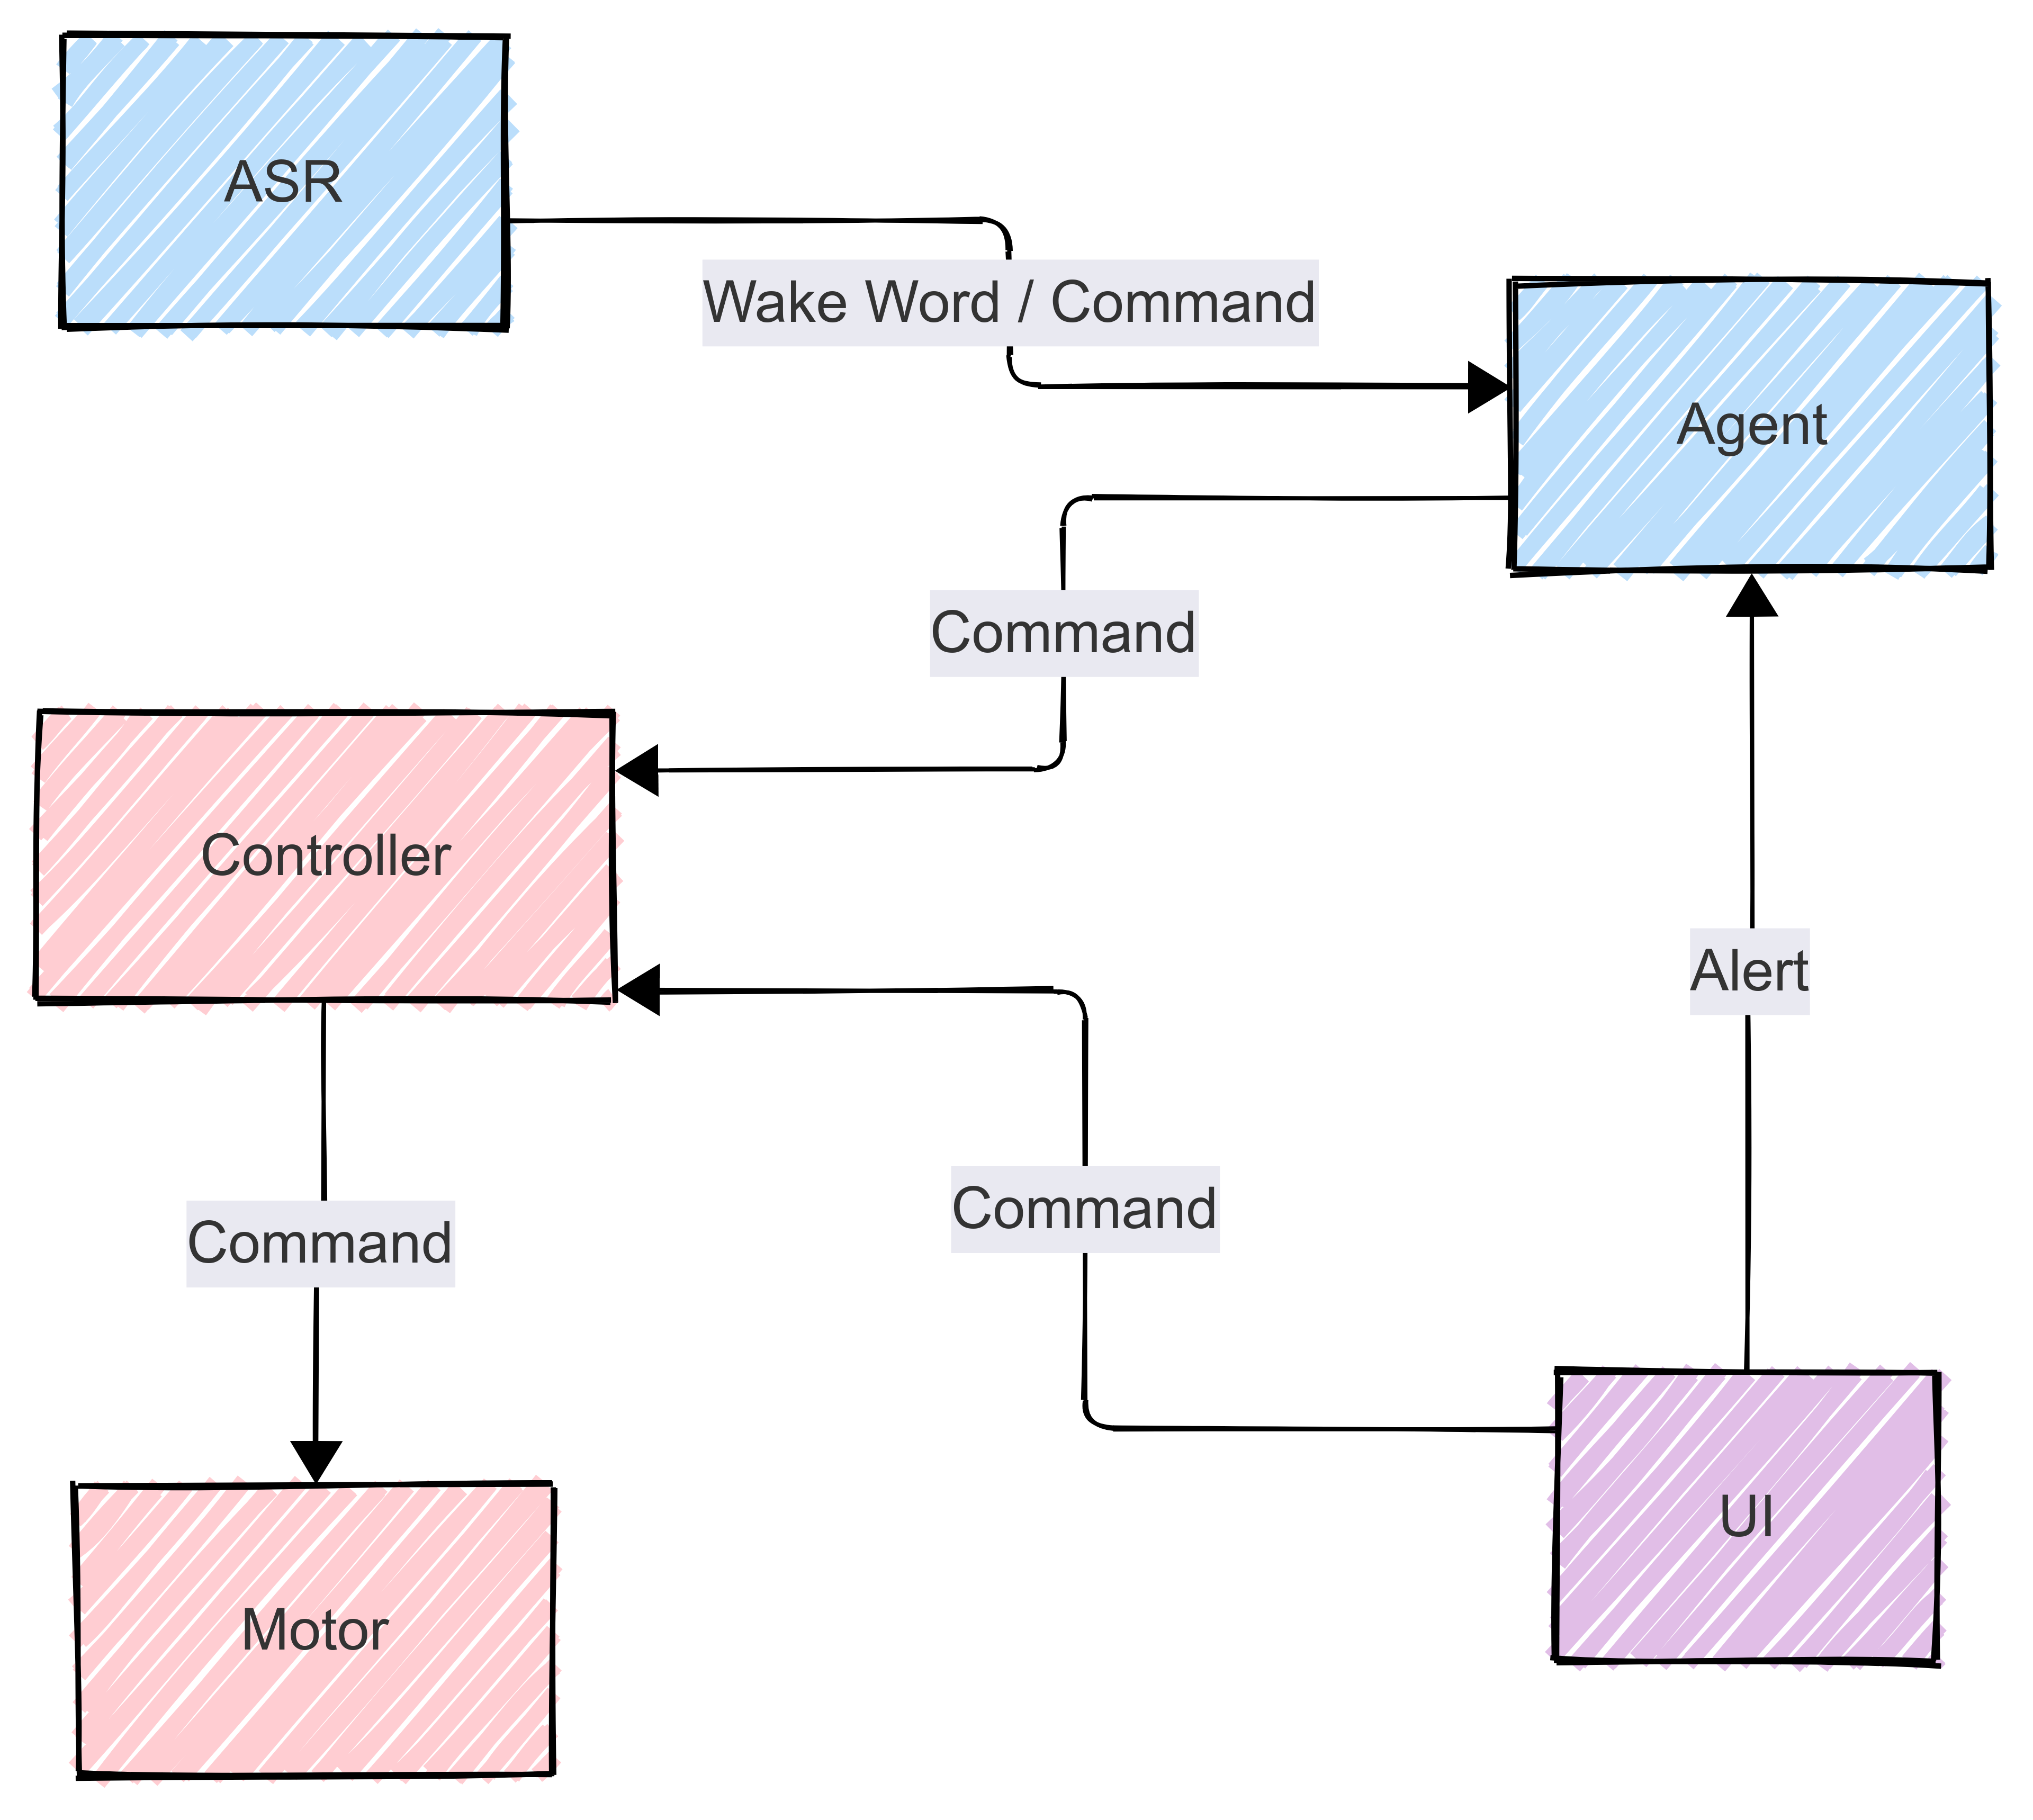
\includegraphics[width=\textwidth]{docs/command_flow.png}
    \caption{Command Message Flow}
\end{figure} 

\begin{figure}[H]
    \centering
    \label{fig:graph}
    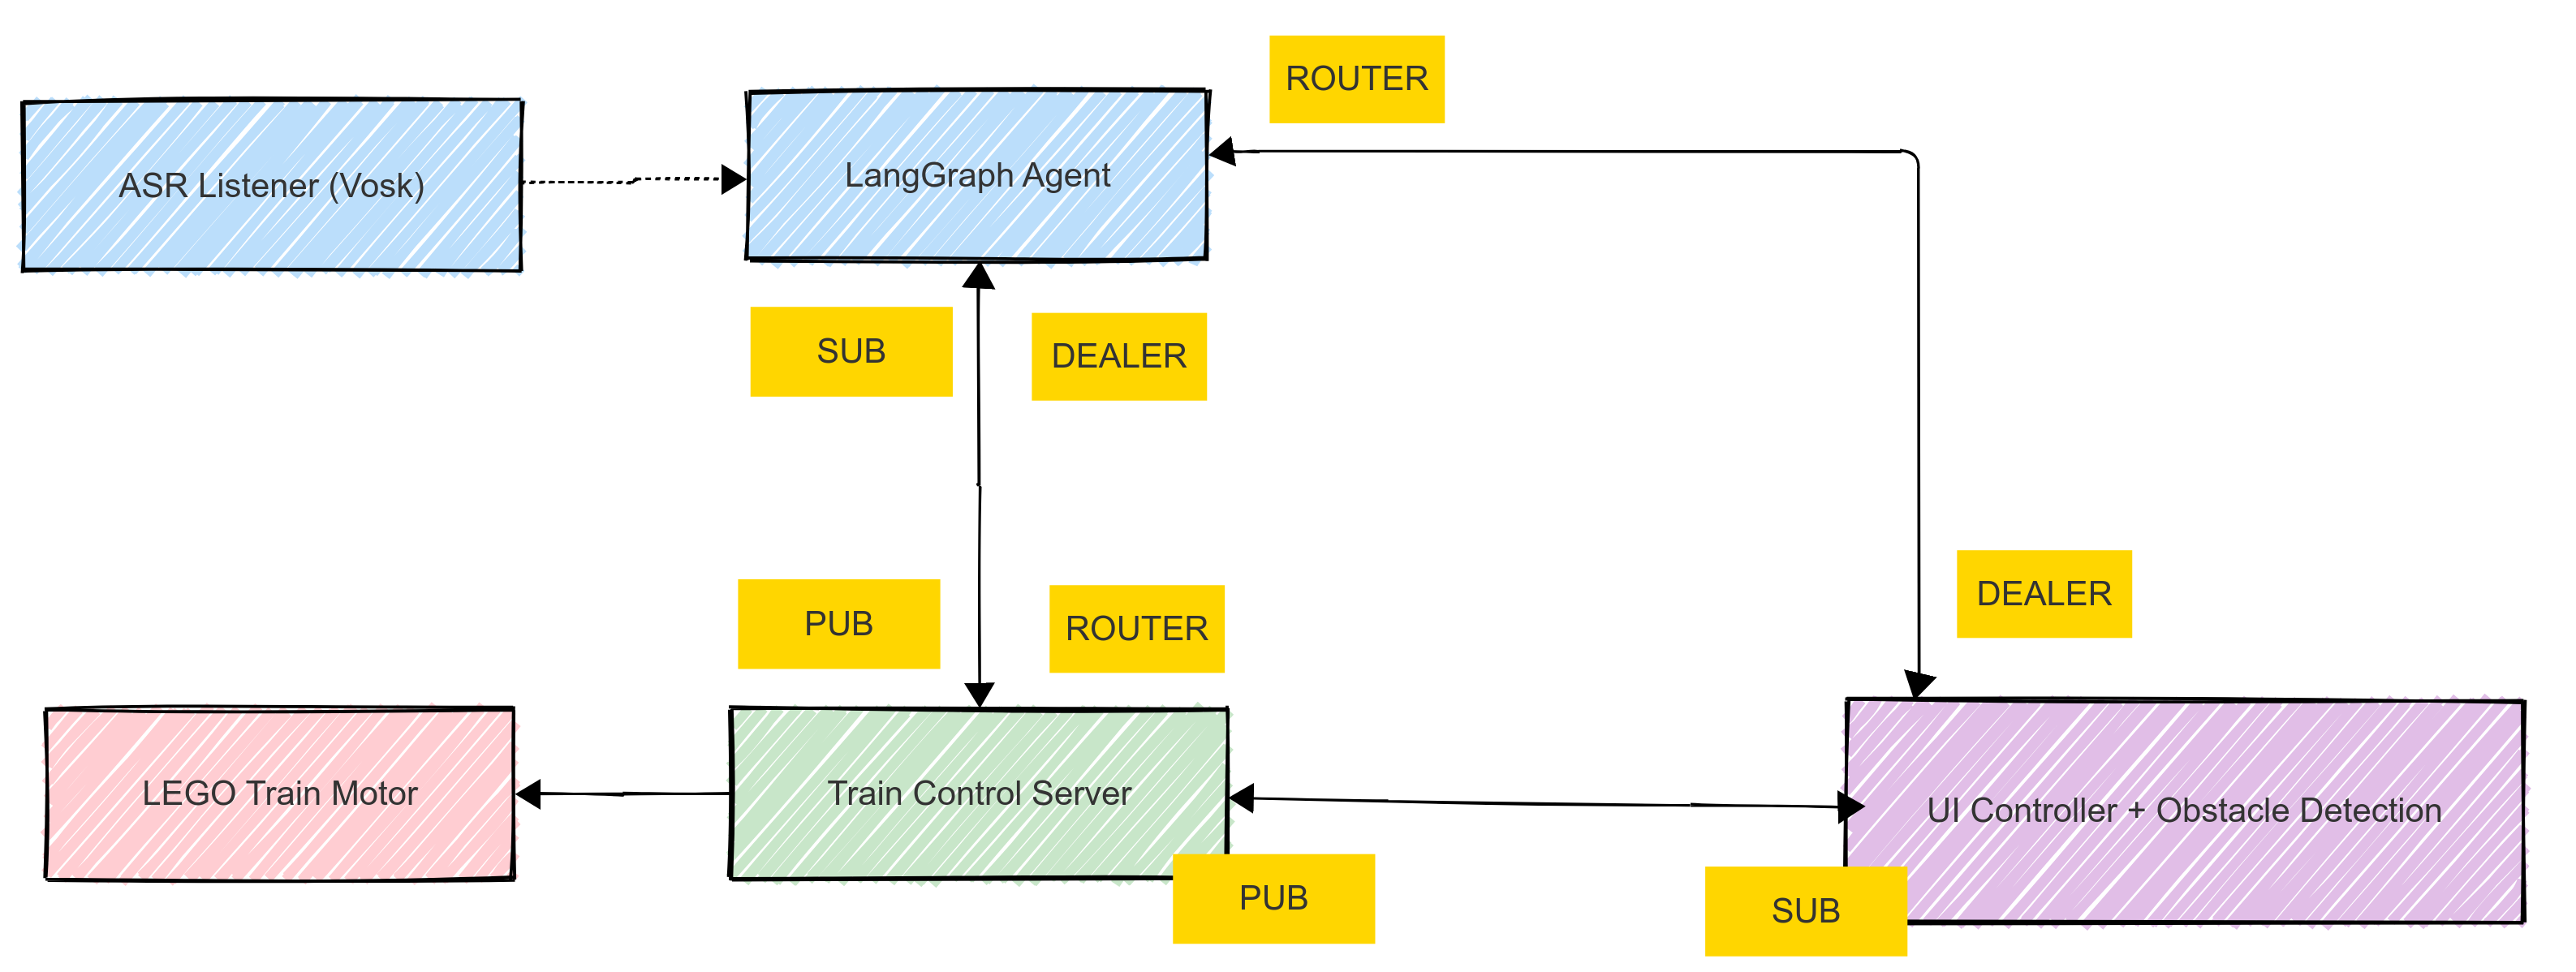
\includegraphics[width=\textwidth]{docs/mqzt flow.png}
    \caption{Message Flow over ZeroMQ}
\end{figure}

The system architecture \ref{fig:system_architecture} of our proposed solution is composed of five components to create an integrated and responsive system:

\begin{itemize}
    \item \textbf{LangGraph-based Agent:} interprets voice/text commands and executes tool functions. 
    \item \textbf{Train Control Server:} interfaces with LEGO motor hardware through the Build Hat module.
    \item \textbf{UI Controller:} handles object detection, displays real-time visual feedback, and control buttons.
    \item \textbf{ZeroMQ Network Layer:} manages asynchronous message passing across the modules in the system.
    \item \textbf{ASR Listener:} processes local speech commands using Vosk.
\end{itemize}




% -------------------------------------
\subsection{LangGraph-Based AI Agent}

The LangGraph framework was chosen for its modular, reactive architecture. It builds on Langchain, which only allows directed cyclic execution and has limited memory. Unlike monolithic agents, LangGraph encodes the workflow including tool execution and autonomous decision-making into a visualizable graph \ref{fig:graph}. The Nodes in the graph represent either LLM reasoning steps or tool invocations, i.e. nodes are actions in a workflow; transitions between them are the edges. Edges can be conditional; therefore, the path is not set. The agent is responsible for interpreting user commands and invoking appropriate tools, all within a cycle of LLM reasoning and external execution. The state in the graph acts as a central control room that all nodes can access and modify.

\begin{figure}[H]
    \centering
    \label{fig:graph}
    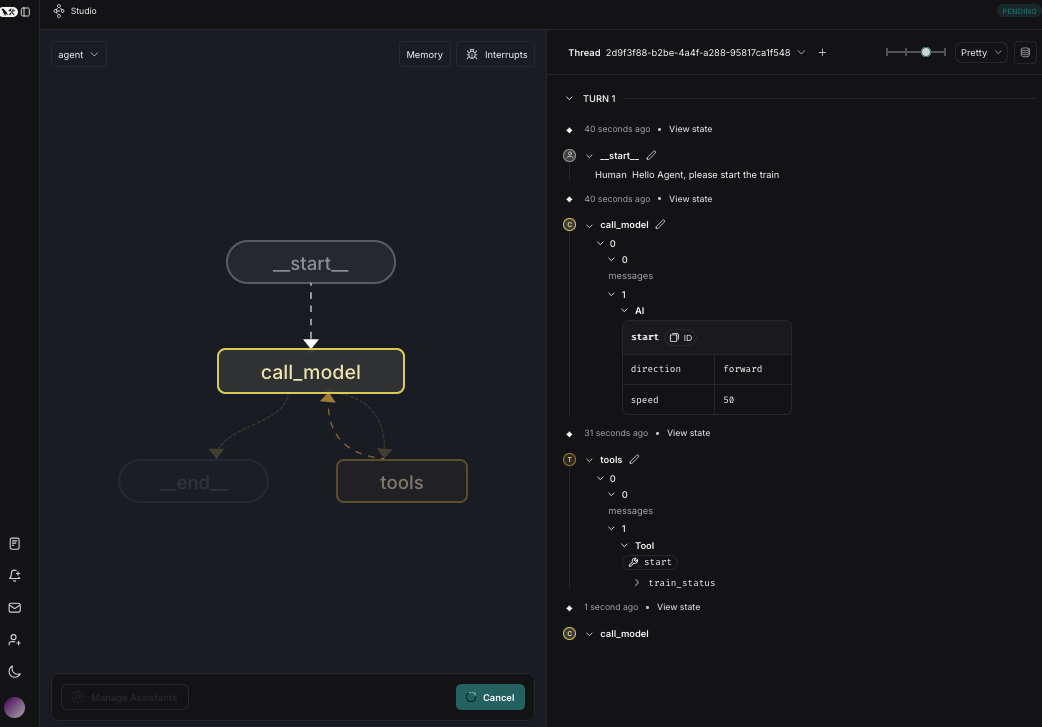
\includegraphics[width=\textwidth]{docs/agent_graph.png}
    \caption{AI Agent Graph}
\end{figure}

Think of Langchain as a one-way train, which has to take a specific route (edges), stopping at different stations (nodes) to do tasks like picking up packages, sorting them, and delivering them to the final destination. While this train can remember what happened during its current journey, it is not very good at remembering things from previous trips. It is perfect for when you know exactly what order you want things to happen in. 

In contrast, LangGraph is a magical train network where trains can travel in any direction and can even travel in circles to visit the same station multiple times. Additionally every station has access to a magical notebook (called the "state") where they can write down and read important information, helping them remember everything that is happening. This makes LangGraph perfect for being like a helpful conductor who can handle lots of different passenger requests in any order and always knows what is going on, even if they need to go back to previous stations.

\begin{lstlisting}[language=Python, caption=AI Controller - Graph Flow]
    builder = StateGraph(State, input=InputState, config_schema=Configuration)
    builder.add_node("call_model", call_model)
    builder.add_node("tools", ToolNode(TOOLS))
    builder.add_edge("__start__", "call_model")
    builder.add_conditional_edges("call_model", route_model_output)
    builder.add_edge("tools", "call_model")
    # ----------------------------------
    # Compile graph into an executable graph
    # You can customize this by adding runtime interrupt points for state updates
    # ----------------------------------
    graph = builder.compile(
    interrupt_before=[],  # Add node names here to UPDATE STATE before they're called
    interrupt_after=[],  # Add node names here to UPDATE STATE after they're called
    )

    graph.name = "AI Train Control Agent"  # This customizes the name in LangSmith for Tracking
\end{lstlisting}


\subsection{Train Control Server}

This server directly controls the LEGO motor using the Build HAT module for the Raspberry Pi. It uses the ZeroMQ \texttt{ROUTER} pattern to accept command requests from AI Agent and UI Controller. On the other hand, it uses the \texttt{PUB} pattern to broadcast train status updates to all participants in the system, but only if the status changed, to ensure that resources are appropriately used. 

\begin{lstlisting}[language=Python, caption=Motor control functions]
    # --------------------------------------
    # Motor control functions
    # --------------------------------------
    def start(self, speed, direction):
        self.is_running = True
        self.direction = direction
        # NOTE negative to mimic backward
        self.speed = speed if self.direction == "forward" else -speed 
        self.train.start(self.speed)  # Start motor with given speed
        print(f"Train Motor started at {self.speed} km/h")

\end{lstlisting}


The Train Control server is always listening for command requests and emits an updated train status after every successful action.

\begin{lstlisting} [language=Python, caption=Train Control Server communication interface]
# -----------------------------------------------------------------------------
# Function: train_control_server
#   For receiving and processing commands from the client (UI and AI Agent).
#   For publishing Train status updates in real-time to all subscribers (UI and AI Agent).
# -----------------------------------------------------------------------------
def train_control_server():

    legoTrainControl = LegoTrainControl()
    print("Train Control Server started, waiting for commands...")

    while True:
        try:
            # Non-blocking receive execution requests
            client_id, empty, request = router_socket.recv_multipart(flags=zmq.NOBLOCK)
            print(f" Received request from {client_id}: {request}")
            try:
                request_data = json.loads(request.decode())
                command = request_data["command"]
                args = request_data.get("args", [])  # Convert JSON args back to Python list

                if not command:
                    raise ValueError("Missing 'command' in request.")
                print(f" Received Request command: {command} with args: {args} from {client_id}.")

                """ Execute the received Command """
                process_command(legoTrainControl, command, args)

                """ Send execution confirmation """
                reply = json.dumps({
                    "request": "executed",
                    "train_status": legoTrainControl.get_status()
                })
                router_socket.send_multipart([client_id, b"", json.dumps(reply).encode()])
                print("Sent execution confirmation.")

                """ Broadcast the train Status, only if changed """
                if legoTrainControl.has_status_changed():
                    status_update = json.dumps({
                        "request": "update",
                        "train_status": legoTrainControl.get_status()
                    })
                    print(f" STATUS UPDATE BROADCAST : {status_update}.")
                    pub_socket.send_string(status_update)

            except (json.JSONDecodeError, ValueError, KeyError) as e:
                error = {
                    "request": "error",
                    "message": f"Invalid request: {str(e)}"
                }
                router_socket.send_multipart([client_id, b"", json.dumps(error).encode()])
                print(f"[ERROR] Bad request: {request} - {e}  - sent back")

        except zmq.Again:
            pass  # No incoming request, continue loop

\end{lstlisting}

\subsection{User Interface and Object Detection}

The UI Controller provides camera-based visual feedback and emergency detection. Obstacle detection is wired directly into the UI loop using TensorFlow Lite. Object detection on the track triggers an alert to the AI agent via ZeroMQ.

\begin{lstlisting}[language=Python, caption=Triggering alerts from UI]
if detected_object['confidence'] > 0.6:
    self.send_alert_command(detected_object)
\end{lstlisting}

This ensures the safety mechanism operates independently from the visual observation loop.

\subsection{ZeroMQ Messaging Layer}



ZeroMQ was selected for its low-latency, modular, and broker-less design. The following patterns are used:

\begin{itemize}
    \item \textbf{DEALER/ROUTER:} for bi-directional commands between UI and Agent
    \item \textbf{DEALER/ROUTER:} for bi-directional commands between UI/Agent and the train controller
    \item \textbf{PUB/SUB:} for broadcasting train status to all components
\end{itemize}

We implemented a central PersistentSocketManager class to handle comminication administration at  one place. This also enables us to cleanly start the background tasks such as connection monitoring and the configuration of the sockets. Furthermore, it realizes proper a cleanup routine.
\begin{lstlisting}[language=Python, caption=Snipped from socket manager]
# Check if we already have a socket with this identity
    existing_socket = PersistentSocketManager.get_socket(identity)
    if existing_socket:
        debug_log(f"[ZMQ SETUP] Reusing existing socket for {identity.decode()}")
        return existing_socket

    # Create a new socket
    context = zmq.Context.instance()
    dealer = context.socket(zmq.DEALER)
    dealer.setsockopt(zmq.IDENTITY, identity)

    # Socket configuration with generous timeouts
    dealer.setsockopt(zmq.HEARTBEAT_IVL, 2000)
    dealer.setsockopt(zmq.HEARTBEAT_TIMEOUT, 10000)
    dealer.setsockopt(zmq.SNDTIMEO, 30000)  # 30 second timeout
    dealer.setsockopt(zmq.RCVTIMEO, 30000)  # 30 second timeout
\end{lstlisting}


\subsection{Always-On ASR with Vosk}

Speech input is processed using Vosk for offline ASR in the \texttt{asr\_stream.py} and the delivery of the transcript to the Agent is cleanly separately through \texttt{agent\_interface.py}. Wake word detection filters irrelevant audio, avoiding noisy LLM queries.

\begin{lstlisting}[language=Python, caption=Wake-word filtering]
# Ignore any text immediately after wake word detection to avoid
                    # processing "hey agent" itself as a command
                    if current_time - wake_word_time < COMMAND_DELAY:
                        buffered_commands.append(text)
                        debug_log(f"Buffered text: {text}")
                        continue

                    # Skip if the text is just the wake word
                    if text == WAKE_WORD or text == "agent" or text == "hey":
                        debug_log(f"Skipping wake word as command: {text}")
                        continue
\end{lstlisting}

Once active, transcribed commands are passed to the LangGraph entry node for further reasoning and tool invocation.

\subsection{Tool Functions and Runtime State Sync}

Agent tools encapsulate train commands like \texttt{start()}, \texttt{stop()}, \texttt{get\_status()}. The graph runtime State is governed centrally, and is injected to the ToolNodes automatically. 

\begin{lstlisting}[language=Python, caption=Train control tool call]
async def start(speed: int, direction: str) -> dict:
    result = await send_train_command("start", [speed, direction])
    return {"train_status": result}
\end{lstlisting}

However, background tasks like the broadcast listener, cant access the State. Therfore we defined our custom \texttt{RuntimeState}. Now the listener can inject the newly received train status data into this. The \texttt{RuntimeState} singleton synchronizes the state between components, ensuring coherent execution even with asynchronous delays.

\subsection{Startup Pattern and Background Threads}

All side-effect logic is centralized in \texttt{startup.py}, including listener registration, ASR thread launch, and ZeroMQ initialisation.

\begin{lstlisting}[language=Python, caption=Startup orchestration]
start_ui_listener()
start_asr_listener()
start_train_status_listener()
\end{lstlisting}

This clean design allows the agent logic to remain pure and testable, and simplifies shutdown and reinitialization.

\section{Implementation Considerations and Best Practices}
\label{sec:impl-bestpractices}

One of the main architectural principles I followed in this project was a strict separation of concerns. This helped keep things modular and debuggable—especially as the system grew more complex. Here’s how I approached that.

\subsection{Modular Feature Encapsulation}

Each part of the system, ASR, agent logic, motor control, UI feedback, and the safety mechanism, was implemented in a separate Python module. This made everything easier to test and also easier to explain when showing the system to others. It also means students or educators can explore individual subsystems without needing to run the full pipeline.

The agent is entirely focused on reasoning and tool calling. I made sure all other logic in the system stayed where it belonged. This kind of modularity reflects how real-world AI services are built—and helped me avoid a lot of circular import bugs.

\subsection{Centralized Communication Configuration}

I moved all the ZeroMQ socket setup and monitoring into a shared utility module. That way, if I needed to tweak timeouts, heartbeats, or reconnect behavior, I could do it in one place. It also helped reduce message desync and ensured the same behavior across all components.

\begin{lstlisting}[language=Python, caption={ZeroMQ socket configuration (excerpt)}]
# From react_agent/utils/zmq_socket.py
socket.setsockopt(zmq.LINGER, 0)
socket.setsockopt(zmq.RECONNECT_IVL, 2000)
socket.setsockopt(zmq.RCVTIMEO, 500)
\end{lstlisting}

I adjusted these options through trial and error while running the system on the Raspberry Pi, trying to find settings that worked under load.

\subsection{Startup Logic and Background Event Loop}

To avoid unexpected side effects during imports, I created a single `startup.py` script as the only entry point. It launches all asynchronous background listeners—like the UI relay, train status monitor, and ASR voice stream. This helped me avoid a lot of issues with async event loops conflicting with LangGraph’s own internal logic.

\subsection{Fail-Safe Design and Error Resilience}

All my tool functions include basic error handling, retry logic, and state protection. I used a singleton class called `RuntimeState` to share train status safely between threads, like the UI and the agent. Without this, the agent and the GUI could easily get out of sync.

\begin{lstlisting}[language=Python, caption={Runtime-safe state update}]
# From runtime_state.py
class RuntimeState:
    _lock = threading.Lock()
    _train_status: Dict[str, Any] = {}

    @classmethod
    def set_train_status(cls, status: Dict[str, Any]):
        with cls._lock:
            cls._train_status = status.copy()
\end{lstlisting}

This design allowed me to keep the components decoupled, but still consistent, even if a few messages were delayed or dropped.



\section{Educational Practices and Insights}

This project was also designed with students in mind—especially for the upcoming KinderCampus workshops. I took inspiration from constructivist learning theories, like Papert’s “learning by making” and Vygotsky’s idea of building knowledge through guided exploration \cite{papert1980mindstorms}.

Working on a constrained device like the Raspberry Pi forces you to make real engineering trade-offs. There's no GPU, memory is tight, and inference time really matters. These constraints actually make it a perfect teaching tool.

From a pedagogical perspective, the system was designed to support modular experimentation. Threfore the codebase intentionally mirrors good modular software engineering principles to enhance its use in educational contexts. Each subsystem—ASR, UI, controller, LangGraph agent—is independently testable. 
The use of ZeroMQ enables students to build or modify components without reworking the full stack. Each script was tested in isolation to ensure independent reproducibility. 

One of my goals was to make the system readable and tweakable for other students. That’s why I kept logs verbose, made error handling visible, and avoided hiding logic behind complex wrappers. The idea is that this system can be reused as both a sandbox and a real learning platform.

This system is well-suited for future deployment in the University’s KinderCampus outreach program. 
Some of the potential key concepts students could explore include:

\begin{itemize}
    \item \textbf{Agent Architecture:} How LLMs interact with tools to stay safe and useful.
    \item \textbf{Real-Time Control:} How the system reacts to obstacles while still running inference and UI updates.
    \item \textbf{Voice Interaction:} Offline ASR models like Vosk show where the limits are in latency and accuracy.
    \item \textbf{Async Communication:} ZeroMQ helps connect everything—and understanding that is a real skill.
      \item \textbf{Visualizing ZeroMQ} message passing between UI and train control
    \item \textbf{Testing in Pieces:} By isolating each subsystem, it’s easier to test, debug, and learn what each part does.
\end{itemize}

\subsubsection*{Suggested Student Exercises}

\begin{enumerate}
    \item \textbf{Modify the `change\_speed` Tool:} Add a percentage-based adjustment instead of fixed speeds.
    \item \textbf{Measure System Latency:} Track the delay from a voice command to motor actuation under CPU load.
    \item \textbf{Add a LangGraph Branch:} Implement a reasoning path where the agent checks both speed and obstacle status before acting.
    \item \textbf{Simulate Communication Failures:} Drop messages between UI and agent and observe how the system reacts.
    \item \textbf{Change the Wake Word:} Update the ASR to listen for a different word and compare detection reliability.
    
\end{enumerate}

By combining hands-on tinkering with real-world constraints, this project gives students an authentic way to learn about AI, robotics, and system design. It turns abstract ideas into something tangible—and hopefully, fun to explore.


\section{Limitations}

\begin{itemize}
  \item The agent currently lacks structured memory and long-term planning features.
  \item ASR quality drops sharply in noisy environments without noise cancellation.
  \item Safety features rely on rule-based thresholds; advanced AI-based avoidance is out of scope.
  \item Performance is sensitive to system temperature; long-running inference tasks raise CPU load.
\end{itemize}

In Summary, this architecture prioritizes safety, modularity, and transparency while operating under embedded constraints. Though the implementation is incomplete in a few areas (e.g., advanced agent memory), it lays a solid foundation for future educational deployment and system scalability.\\

The proposed agentic system on the Raspberry Pi provides several notable advantages:

\begin{itemize}
    \item \textit{Enhanced Reasoning Capability}: The integration of the LangGraph framework allows the agent to reason through commands, offering intelligent responses that go beyond the execution of simple commands. It can understand the context and history of previous interactions, improving the overall user experience.

    \item \textit{State Management and Safety}: The agent's ability to keep track of the train's operational state enhances safety. This allows for dynamic changes based on both user commands and real-time environmental conditions like obstacles.

    \item \textit{Accessibility}: The combination of ASR and LLM makes the system accessible to a broader audience, allowing users with varying levels of technical expertise to interact with the LEGO train system easily.

    \item \textit{Cost-effective and Open-Source}: The use of Raspberry Pi as the central platform alongside open source tools reduces the overall cost barrier for development and implementation. This encourages experimentation and customization within educational and hobbyist communities.
\end{itemize}